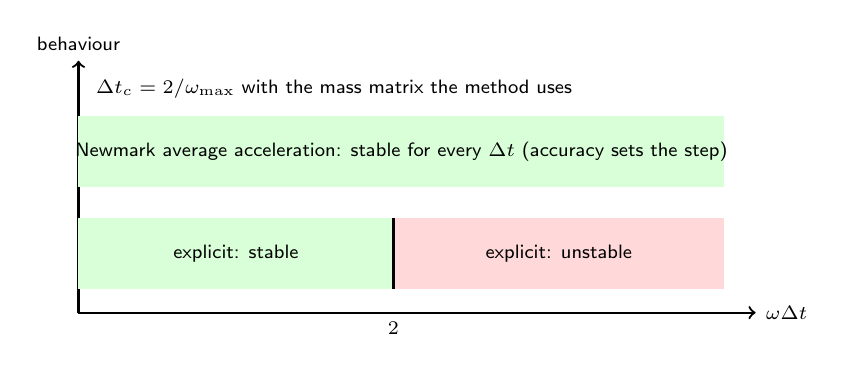
\begin{tikzpicture}[font=\sffamily\scriptsize]
\draw[->,thick] (0,0) -- (8.6,0) node[right] {$\omega\Delta t$};
\draw[->,thick] (0,0) -- (0,3.2) node[above] {behaviour};
\fill[green!15] (0,0.3) rectangle (4.0,1.2);
\fill[red!15] (4.0,0.3) rectangle (8.2,1.2);
\draw[thick] (4.0,0.3) -- (4.0,1.2);
\node at (2.0,0.75) {explicit: stable};
\node at (6.1,0.75) {explicit: unstable};
\node[below] at (4.0,0) {$2$};
\fill[green!15] (0,1.6) rectangle (8.2,2.5);
\node at (4.1,2.05) {Newmark average acceleration: stable for every $\Delta t$ (accuracy sets the step)};
\node[align=left,anchor=west] at (0.1,2.85) {$\Delta t_c=2/\omega_{\max}$ with the mass matrix the method uses};
\end{tikzpicture}
